\documentclass[aspectratio=169,12pt]{beamer}
\usetheme[progressbar=none,sectionpage=none]{moloch}
\geometry{paperwidth=320mm,paperheight=180mm}
\usepackage[spanish]{babel}
\shorthandoff{"}
\usepackage{tikz,graphicx,listings,pgfpages}
\usetikzlibrary{arrows.meta}
\usepackage{estilo-sandbox}
\title{Sandbox y permisos en Codex}
\author{Knowledge Sharing}
\hypersetup{pdftitle={Sandbox y permisos en Codex},pdfsubject={Conceptos, fronteras de ejecución y configuración interpretada},pdfauthor={Knowledge Sharing},colorlinks=true,urlcolor=Azul}
\newcommand{\refprincipal}{\url{https://learn.chatgpt.com/docs/sandboxing?surface=app}}
\newcommand{\refseguridad}{\url{https://learn.chatgpt.com/docs/agent-approvals-security}}
\newcommand{\refconfig}{\url{https://learn.chatgpt.com/docs/config-file/config-reference}}
\newcommand{\refauto}{\url{https://learn.chatgpt.com/docs/sandboxing/auto-review}}
\begin{document}

\begingroup
\oscuro
\begin{frame}[plain]
\begin{tikzpicture}[remember picture,overlay,x=1mm,y=1mm]
\begin{scope}[shift={(current page.south west)}]
\pie{01 / Fundamentos}
\texto{16}{166}{160}{11}{\textcolor{Azul}{\textbf{AUTONOMÍA CON LÍMITES}}}
\texto{16}{145}{165}{38}{\textbf{Sandbox y\\permisos en Codex}}
\texto{16}{96}{150}{18}{El sandbox aplica límites técnicos a los comandos que ejecuta Codex.}
\texto{16}{61}{150}{15}{Define qué archivos pueden leer o modificar y qué conexiones de red pueden realizar.}
\texto{187}{137}{115}{16}{\textcolor{Azul}{\textbf{Ejemplo: guardar un informe}}}
\draw[limite] (181,77) rectangle (305,119);
\texto{188}{111}{111}{15}{Dentro del proyecto\\\texttt{resultados/informe.json}}
\texto{188}{87}{111}{12}{Escritura autorizada}
\texto{188}{61}{111}{15}{En otra carpeta\\Puede requerir una excepción}
\texto{181}{29}{124}{10}{Ejemplo de escritura limitada al proyecto y temporales autorizados.}
\note{El sandbox de Codex limita técnicamente la ejecución de comandos. No es una instrucción de buen comportamiento escrita en el prompt. Introducir primero archivos y red, sin exigir vocabulario de procesos. El ejemplo ilustra escritura en el proyecto; no afirma que todas las lecturas estén limitadas a él. Una excepción depende de las políticas y no está siempre disponible. Fuentes oficiales consultadas el 6 de noviembre de 2026: \refprincipal\ y \refseguridad.}
\end{scope}
\end{tikzpicture}
\end{frame}
\endgroup

\begin{frame}[plain]
\begin{tikzpicture}[remember picture,overlay,x=1mm,y=1mm]
\begin{scope}[shift={(current page.south west)}]
\pie{01 / Fundamentos}
\tit{Una tarea permite ver los límites}
\bajada{Petición: «Evalúa seis casos y guarda un informe».}
\texto{20}{123}{280}{12}{Política ilustrativa: escritura en el proyecto y temporales; red de comandos desactivada.}
\node[anchor=north west] at (20,106) {\begin{minipage}{280mm}
\fontsize{16}{23}\selectfont
\renewcommand{\arraystretch}{1.3}
\begin{tabular}{@{}p{143mm}p{127mm}@{}}
\toprule
\textcolor{Azul}{\textbf{Acción del comando}} & \textcolor{Azul}{\textbf{Qué ocurre}} \\
\midrule
Guardar el informe en el proyecto & Escritura autorizada \\
\midrule
Exportarlo a otra carpeta & Requiere una excepción elegible \\
\midrule
Descargar una dependencia & Necesita acceso de red \\
\bottomrule
\end{tabular}
\end{minipage}};
\cierre{La misma tarea puede incluir acciones permitidas y acciones que requieren revisión.}
\note{Ejemplo resuelto que se mantiene a lo largo del deck. Evaluar seis casos aquí significa ejecutar el evaluador determinista local, no llamar a una API ni a otro modelo. La escritura externa se bloquea bajo la política ilustrativa; puede solicitarse una excepción si las políticas lo permiten. La red desactivada se refiere a los comandos del sandbox, no a las conexiones del cliente con el servicio de Codex ni a toda herramienta. Una acción técnicamente permitida aún puede estar sujeta a otras reglas de aprobación. Fuentes oficiales, consulta del 6 de noviembre de 2026: \refseguridad\ y \url{https://learn.chatgpt.com/docs/permissions}.}
\end{scope}
\end{tikzpicture}
\end{frame}

\begin{frame}[plain]
\begin{tikzpicture}[remember picture,overlay,x=1mm,y=1mm]
\begin{scope}[shift={(current page.south west)}]
\pie{01 / Fundamentos}
\tit{En tu equipo, el sistema aplica los límites}
\bajada{Codex solicita un comando. El programa se ejecuta bajo los controles locales.}
\node[caja,minimum width=65mm] (codex) at (49,101) {Codex solicita\\crear el informe};
\node[caja,minimum width=83mm] (python) at (153,101) {Python intenta\\escribir el archivo};
\node[caja,minimum width=74mm] (sistema) at (270,101) {Sistema operativo\\permite o bloquea};
\draw[flujo] (codex.east) -- (python.west);
\draw[flujo] (python.east) -- (sistema.west);
\texto{20}{73}{133}{14}{\textcolor{Azul}{\textbf{Ejecución local}}\\Los comandos corren en tu equipo.\\El sandbox puede usar controles del sistema, sin una máquina virtual.}
\texto{174}{73}{130}{14}{\textcolor{Azul}{\textbf{Ejecución cloud}}\\Los comandos corren en un entorno remoto con sus propios permisos.}
\cierre{Los permisos de navegador, búsqueda y conectores se controlan por separado.}
\note{El diagrama explica ejecución local de comandos, no toda la arquitectura de Codex. El agente usa un modelo para decidir y una herramienta para iniciar Python, Git u otros programas. El sistema operativo impone las restricciones aplicables. En macOS se utilizan políticas Seatbelt; en Linux, mecanismos como bubblewrap y seccomp. Los detalles de plataforma permanecen en notas. Un sandbox no equivale siempre a una VM ni a un contenedor. Las ejecuciones cloud tienen su propio entorno. Navegador, búsqueda, MCP y conectores no heredan universalmente los controles del shell local. Fuentes oficiales consultadas el 6 de noviembre de 2026: \refseguridad\ y \url{https://learn.chatgpt.com/docs/permissions\#scope-and-enforcement}.}
\end{scope}
\end{tikzpicture}
\end{frame}

\begin{frame}[plain]
\begin{tikzpicture}[remember picture,overlay,x=1mm,y=1mm]
\begin{scope}[shift={(current page.south west)}]
\pie{01 / Fundamentos}
\tit{Al empezar, comprueba los permisos efectivos}
\bajada{En un repositorio confiable, el inicio habitual permite trabajar dentro del proyecto.}
\texto{20}{121}{133}{17}{\textcolor{Azul}{\textbf{Inicio habitual: Auto}}}
\texto{20}{101}{136}{14}{\texttt{workspace-write}\\Escritura en el proyecto y temporales autorizados.}
\texto{20}{73}{136}{14}{\texttt{on-request}\\Revisión cuando una acción necesita aprobación.}
\texto{20}{45}{136}{13}{Red de comandos desactivada por defecto.}
\draw[Linea,line width=.5pt] (163,43) -- (163,125);
\texto{179}{121}{124}{17}{\textcolor{Azul}{\textbf{Compruébalo en CLI}}}
\texto{179}{100}{124}{15}{\texttt{/status}\\Consultar el estado de la sesión.}
\texto{179}{74}{124}{15}{\texttt{/permissions}\\Consultar o cambiar permisos.}
\texto{179}{47}{124}{12}{Una carpeta sin confianza puede iniciar en solo lectura.}
\cierre{La configuración, el cliente y las políticas pueden cambiar estos valores.}
\note{Valores habituales, no afirmación sobre todas las sesiones. La documentación indica que al detectar control de versiones Codex recomienda Auto, con workspace-write y on-request; sin control de versiones recomienda read-only. Algunos entornos empiezan en read-only hasta confiar explícitamente en el directorio. La confianza no sustituye los controles técnicos. La configuración y los requisitos administrados determinan el resultado efectivo. /status y /permissions se presentan como comandos del CLI, no controles universales de todas las superficies. workspace-write no restringe automáticamente todas las lecturas al proyecto. Sus raíces conservan subrutas protegidas como .git, .codex, .agents y .aws. Fuentes oficiales, consulta del 6 de noviembre de 2026: \refseguridad\ y \url{https://learn.chatgpt.com/docs/agent-approvals-security\#defaults-and-recommendations}.}
\end{scope}
\end{tikzpicture}
\end{frame}

\begin{frame}[plain]
\begin{tikzpicture}[remember picture,overlay,x=1mm,y=1mm]
\begin{scope}[shift={(current page.south west)}]
\pie{01 / Fundamentos}
\tit{Exportar fuera del proyecto puede necesitar revisión}
\bajada{El informe ya existe. Codex intenta copiarlo a una carpeta de entregas externa.}
\node[caja,minimum width=78mm] (informe) at (57,105) {Informe dentro\\del proyecto};
\node[caja,minimum width=79mm] (exportar) at (164,105) {Escritura fuera\\del alcance ordinario};
\node[caja,minimum width=63mm] (solicitud) at (276,105) {Solicitud de\\excepción elegible};
\draw[flujo] (informe.east) -- (exportar.west);
\draw[flujo] (exportar.east) -- (solicitud.west);
\texto{20}{75}{135}{14}{\textcolor{Azul}{\textbf{Sandbox}}\\Restringe la escritura externa con los permisos actuales.}
\texto{177}{75}{128}{14}{\textcolor{Azul}{\textbf{Revisión}}\\Evalúa la acción, el destino y su autorización. Puede aprobar o denegar.}
\texto{20}{43}{284}{12}{Si la política no permite solicitar una excepción, la acción se detiene.}
\cierre{Aprobar una excepción puede ampliar esa ejecución; no concede acceso general.}
\note{El ejemplo usa la misma exportación que la demo. No implica que cualquier bloqueo técnico siempre produzca una solicitud de aprobación: depende del cliente y de las políticas. Primero se explica el límite técnico y después la revisión. Una aprobación puede ampliar el alcance de esa ejecución. Una denegación exige detener esa acción o elegir una alternativa autorizada, no eludirla. Las reglas de comandos pueden añadir revisión y el revisor puede ser humano o automático. Fuentes oficiales, consulta del 6 de noviembre de 2026: \refseguridad\ y \refauto.}
\end{scope}
\end{tikzpicture}
\end{frame}

\begingroup
\oscuro
\begin{frame}[plain]
\begin{tikzpicture}[remember picture,overlay,x=1mm,y=1mm]
\begin{scope}[shift={(current page.south west)}]
\pie{02 / Auto-review}
\tit{Cuándo interviene Auto-review}
\bajada{Las acciones sin aprobación adicional continúan. Las solicitudes elegibles se revisan.}

\node[caja,minimum width=60mm] (accion) at (47,92) {Acción propuesta};
\node[caja,minimum width=65mm] (solicitud) at (144,92) {¿Aprobación?};
\node[caja,minimum width=85mm] (continua) at (264,118) {Continúa};
\node[caja,minimum width=85mm] (revisa) at (264,76) {Usuario o Auto-review};
\draw[flujo] (accion.east) -- (solicitud.west);
\draw[flujo] (solicitud.east) -- (201,92) |- (continua.west);
\draw[flujo] (201,92) |- (revisa.west);
\texto{203}{131}{17}{11}{No}
\texto{187}{66}{116}{11}{Sí: solicitud elegible, según la política}
\texto{20}{49}{280}{12}{Ejemplo: exportar el informe a una carpeta de entregas fuera del alcance actual.}
\texto{20}{36}{280}{12}{La política debe permitir solicitar esa excepción. No se anticipa la decisión.}
\cierre{Auto-review evalúa solicitudes de aprobación elegibles.}

\note{El flujo se limita a acciones que pueden continuar sin aprobación o generar una solicitud elegible. No muestra como aprobables todas las acciones fuera del alcance: algunas restricciones no admiten excepción, como ya se explicó en el flujo general. Con approvals\_reviewer = auto\_review y una política interactiva como on-request, las solicitudes elegibles llegan al agente revisor; con user, al usuario. Una regla explícita puede exigir revisión de una acción sensible incluso dentro del sandbox. Computer Use mantiene aprobaciones de aplicaciones propias. El caso de /ruta/entregas es conceptual y no se ejecuta ni se asume aprobado. Contraste: una edición ya permitida y sin revisión adicional continúa sin activar Auto-review. Pregunta: ¿revisa toda acción? No. Con never no hay solicitudes para revisar. Fuentes oficiales, consulta del 5 de noviembre de 2026: \refauto\ y \refseguridad.}

\end{scope}
\end{tikzpicture}
\end{frame}
\endgroup

\begin{frame}[plain]
\begin{tikzpicture}[remember picture,overlay,x=1mm,y=1mm]
\begin{scope}[shift={(current page.south west)}]
\pie{02 / Auto-review}
\tit{Qué evalúa el revisor}
\bajada{Un agente separado evalúa la acción exacta con el contexto disponible.}

\draw[limite] (18,68) rectangle (138,122);
\texto{25}{115}{106}{13}{Petición y contexto}
\texto{25}{99}{106}{13}{Acción exacta y destino}
\texto{25}{83}{106}{13}{Evidencia relevante}
\node[caja,minimum width=69mm,minimum height=24mm] (politica) at (190,95) {Evaluación\\según la política};
\node[caja,minimum width=57mm,minimum height=24mm] (resultado) at (280,95) {Decisión y\\explicación};
\draw[flujo] (139,95) -- (politica.west);
\draw[flujo] (politica.east) -- (resultado.west);
\texto{20}{54}{281}{14}{¿Qué se hará? ¿Hay autorización? ¿Qué riesgos y efectos tiene?}
\texto{20}{38}{281}{12}{Ejemplo: identificar la escritura solicitada y su carpeta de destino.}
\cierre{La revisión usa contexto y evidencia. No es una garantía infalible.}

\note{El revisor recibe una transcripción compacta, la solicitud exacta y evidencia relevante de herramientas. Puede realizar comprobaciones de solo lectura para completar contexto; no recibe razonamiento interno privado. En el ejemplo, se identifica qué archivo se escribiría y en qué carpeta, junto con la petición que respalda la acción. La política busca detectar exfiltración de información privada, búsqueda de credenciales, debilitamiento persistente de seguridad y acciones destructivas con riesgo irreversible. Estos son objetivos documentados, no garantías de detección. No inventar una respuesta del revisor ni afirmar qué resultado debe producir el caso conceptual. La política puede variar por configuración y requisitos administrados. Personalizarla puede sustituir su contenido: conservar la política vigente completa y no aplicar plantillas incompletas. Fuentes oficiales, consulta del 5 de noviembre de 2026: \refauto. Diseño segmentado y explicación adyacente adaptados de \url{https://citral.ucsb.edu/faculty/resources/engaging-students/explaining-content}.}

\end{scope}
\end{tikzpicture}
\end{frame}

\begin{frame}[plain]
\begin{tikzpicture}[remember picture,overlay,x=1mm,y=1mm]
\begin{scope}[shift={(current page.south west)}]
\pie{02 / Auto-review}
\tit{Qué ocurre después de la revisión}
\bajada{Aprobación y denegación son decisiones. Un timeout es un fallo técnico.}

\texto{22}{119}{85}{16}{\textcolor{Azul}{\textbf{Aprobación}}}
\texto{118}{119}{183}{14}{Puede continuar la acción\\con el alcance autorizado.}
\regla{96}
\texto{22}{88}{85}{16}{\textcolor{Violeta}{\textbf{Denegación}}}
\texto{118}{88}{183}{14}{Alternativa más segura\\o detenerse y consultar.}
\texto{118}{69}{183}{11}{No eludir el rechazo ejecutando lo mismo por otro camino.}
\regla{58}
\texto{22}{50}{85}{15}{\textcolor{Azul}{\textbf{Timeout}}\\\textcolor{Azul}{\fontsize{10}{12}\selectfont Fallo técnico}}
\texto{118}{50}{183}{13}{La revisión no terminó a tiempo.\\Eso no demuestra que la acción sea insegura.}
\cierre{Aprobar esa acción no concede permisos generales para acciones futuras.}
\texto{12}{13}{295}{9}{Auto-review puede equivocarse. Complementa al sandbox y a las políticas de la organización.}

\note{Al aprobar, continúa la acción conforme al alcance concedido; no afirmar que toda aprobación crea permisos permanentes. Si se deniega, el agente recibe la razón y debe elegir una alternativa materialmente más segura o detenerse y consultar. No puede perseguir el mismo resultado mediante ejecución indirecta para eludir la política. Un timeout se informa por separado y no constituye una evaluación de riesgo negativa. La implementación abierta documenta un circuit breaker ante tres denegaciones consecutivas o diez dentro de las últimas cincuenta revisiones del mismo turno; es un detalle dependiente de versión. En clientes compatibles, /approve permite seleccionar una acción denegada para un reintento específico que sigue sujeto al revisor y puede volver a denegarse según la política. No confundir ese mecanismo con una anulación general. Ajustar raíces acotadas y reglas precisas puede reducir revisiones rutinarias; evitar reglas amplias que borren la frontera. Preguntas de comprensión: ¿un timeout equivale a denegación? No. ¿Auto-review añade carpetas por adelantado? No. ¿Con never recibe solicitudes? No. Los ejemplos de esta lámina son conceptuales; el recorrido real de la demo se resume al final de la presentación. Fuente oficial, consulta del 5 de noviembre de 2026: \refauto.}

\end{scope}
\end{tikzpicture}
\end{frame}

\begin{frame}[plain]
\begin{tikzpicture}[remember picture,overlay,x=1mm,y=1mm]
\begin{scope}[shift={(current page.south west)}]
\pie{03 / Configuración y alcance}
\tit{Configuración inicial explicada}
\bajada{\texttt{\textasciitilde/.codex/config.toml} guarda tus preferencias de inicio.}

\node[anchor=north west] at (16,122) {\begin{minipage}{174mm}\tcbinputlisting{codigo,listing file=ejemplo-config.toml}\end{minipage}};
\texto{202}{116}{104}{13}{\textcolor{Azul}{\textbf{sandbox\_mode}}\\Alcance técnico inicial.}
\texto{202}{94}{104}{13}{\textcolor{Azul}{\textbf{approval\_policy}}\\Cuándo solicitar aprobación.}
\texto{202}{72}{104}{13}{\textcolor{Azul}{\textbf{approvals\_reviewer}}\\Quién revisa las solicitudes.}
\texto{202}{50}{104}{13}{\textcolor{Azul}{\textbf{Raíces y red}}\\Accesos de los comandos.}
\cierre{Ejemplo didáctico. Su efecto está sujeto a la configuración y requisitos efectivos.}

\note{Interpretar antes de comparar: workspace-write permite escritura en raíces autorizadas; on-request permite solicitar aprobación; user dirige revisión al usuario; writable\_roots vacío no añade raíces; network\_access false mantiene deshabilitada la red de comandos dentro de ese sandbox. No se aplica este archivo a la configuración real. Las preferencias personales pueden ser reemplazadas por capas de mayor prioridad, respetando requisitos obligatorios. Un proyecto de confianza puede aportar su .codex/config.toml. No combinar este ejemplo con default\_permissions y tablas de perfiles nuevos. Fuente oficial, consulta del 5 de noviembre de 2026: \refconfig\ y \url{https://learn.chatgpt.com/docs/config-file/config-basic}.}

\end{scope}
\end{tikzpicture}
\end{frame}

\begin{frame}[plain]
\begin{tikzpicture}[remember picture,overlay,x=1mm,y=1mm]
\begin{scope}[shift={(current page.south west)}]
\pie{03 / Configuración y alcance}
\tit{Cambiar una decisión de configuración}
\bajada{Cada comparación parte de la misma base. Solo cambia la línea señalada.}

\texto{20}{118}{281}{13}{\textcolor{Azul}{\textbf{A. Cuándo solicitar aprobación}}}
\texto{20}{101}{281}{14}{\texttt{approval\_policy = \textquotedbl on-request\textquotedbl} $\rightarrow$ \texttt{approval\_policy = \textquotedbl never\textquotedbl}}
\texto{20}{86}{281}{14}{Se eliminan las solicitudes. El sandbox conserva sus límites.}
\regla{73}
\texto{20}{64}{281}{13}{\textcolor{Azul}{\textbf{B. Quién revisa, conservando on-request}}}
\texto{20}{47}{281}{14}{\texttt{approvals\_reviewer = \textquotedbl user\textquotedbl} $\rightarrow$ \texttt{approvals\_reviewer = \textquotedbl auto\_review\textquotedbl}}
\texto{20}{32}{281}{14}{Se delega la revisión elegible. No se amplían las carpetas por ese cambio.}
\texto{12}{15}{290}{10}{Son variantes independientes. Con never no hay solicitudes que auto-review pueda revisar.}

\note{Se muestran las líneas TOML antes y después de cada cambio, con sintaxis completa. A modifica únicamente approval\_policy desde la base. B vuelve a partir de la base con on-request y modifica únicamente approvals\_reviewer. No se aplican A y B consecutivamente. Pregunta: never permite escribir fuera del alcance? No. La política no autoriza por sí sola operaciones denegadas. Fuente oficial, consulta del 5 de noviembre de 2026: \refseguridad\ y \refauto.}

\end{scope}
\end{tikzpicture}
\end{frame}

\begin{frame}[plain]
\begin{tikzpicture}[remember picture,overlay,x=1mm,y=1mm]
\begin{scope}[shift={(current page.south west)}]
\pie{03 / Configuración y alcance}
\tit{Alcance de escritura}
\bajada{writable\_roots añade ubicaciones de escritura al modo workspace-write.}

\draw[limite] (20,78) rectangle (147,120);
\texto{28}{113}{110}{16}{\textcolor{Azul}{\textbf{Proyecto}}}
\texto{28}{94}{110}{12}{Raíces ya autorizadas}
\node[caja,minimum width=112mm] (extra) at (245,99) {/ruta/compartida};
\draw[flujo] (148,99) -- (extra.west);
\texto{20}{66}{285}{13}{\texttt{writable\_roots = []}}
\texto{20}{50}{285}{13}{\texttt{writable\_roots = [\textquotedbl/ruta/compartida\textquotedbl]}}
\texto{20}{34}{285}{12}{Cambia solo la carpeta adicional. La política de aprobación y la red se conservan.}
\texto{12}{16}{290}{10}{Ruta ficticia. workspace-write no limita automáticamente todas las lecturas al proyecto.}

\note{Comparar ambas listas manteniendo el resto de la base. La carpeta adicional no sustituye las raíces del proyecto. La lista vacía tampoco elimina ubicaciones temporales que permita la configuración efectiva. Las rutas protegidas pueden tener reglas propias. Para tareas en repositorios distintos, preferir proyectos o worktrees separados a ampliar de forma general el alcance. Una excepción puntual puede usar revisión acotada o reglas de comando compatibles. No se crea la ruta ficticia ni se cambian permisos. Fuente oficial, consulta del 5 de noviembre de 2026: \refconfig\ y \refprincipal.}

\end{scope}
\end{tikzpicture}
\end{frame}

\begin{frame}[plain]
\begin{tikzpicture}[remember picture,overlay,x=1mm,y=1mm]
\begin{scope}[shift={(current page.south west)}]
\pie{03 / Configuración y alcance}
\tit{Acceso de red}
\bajada{Habilitar conexiones de comandos es distinto de permitir escritura.}

\texto{22}{116}{128}{16}{\textcolor{Azul}{\textbf{Red deshabilitada}}}
\texto{22}{95}{129}{14}{\texttt{network\_access = false}}
\texto{22}{75}{128}{14}{El comando no recibe\\acceso saliente de red.}
\texto{173}{116}{130}{16}{\textcolor{Azul}{\textbf{Red habilitada}}}
\texto{173}{95}{130}{14}{\texttt{network\_access = true}}
\texto{173}{75}{129}{14}{Puede usar red según\\los controles efectivos.}
\draw[Linea,line width=.5pt] (158,57) -- (158,122);
\texto{22}{45}{279}{12}{Ejemplo: descargar una dependencia. El destino puede requerir filtros o autenticación.}
\cierre{Este ajuste no define los permisos de todos los navegadores y conectores.}

\note{Se modifica únicamente network\_access dentro de sandbox\_workspace\_write, conservando las demás claves de la base. Habilitar red no prueba conectividad a todo destino ni anula controles administrados, proxy, firewall o autenticación. Configurar destinos permitidos y activar su mecanismo de filtrado son decisiones distintas que dependen de plataforma y configuración. No afirmar que true aplica por sí solo una allowlist. Pregunta: esta regla bloquea todo navegador cloud? No. La prueba de conectividad no se ejecuta aquí. Fuente oficial, consulta del 5 de noviembre de 2026: \refconfig\ y \refseguridad.}

\end{scope}
\end{tikzpicture}
\end{frame}

\begin{frame}[plain]
\begin{tikzpicture}[remember picture,overlay,x=1mm,y=1mm]
\begin{scope}[shift={(current page.south west)}]
\pie{03 / Configuración y alcance}
\tit{Los modos cambian el alcance de los comandos}
\bajada{Elegir un modo cambia los accesos; la política de aprobación se configura aparte.}
\texto{20}{117}{90}{13}{\textcolor{Azul}{\texttt{read-only}}}
\texto{121}{120}{179}{19}{Lectura bajo controles}
\texto{121}{104}{179}{14}{Las escrituras quedan restringidas.}
\regla{91}
\texto{20}{81}{90}{13}{\textcolor{Azul}{\texttt{workspace-write}}}
\texto{121}{84}{179}{19}{Escritura en el proyecto}
\texto{121}{68}{179}{14}{También en otras ubicaciones autorizadas.}
\regla{55}
\texto{20}{45}{94}{13}{\textcolor{Violeta}{\texttt{danger-full-access}}}
\texto{121}{48}{179}{19}{Sin las fronteras del sandbox}
\texto{121}{32}{179}{14}{Persisten los permisos del sistema.}
\texto{12}{15}{290}{10}{Solo lectura puede permitir ejecutar programas que respeten sus límites.}

\note{La página principal resume read-only con una descripción simplificada de comandos y aprobación. La guía de seguridad aclara que los comandos permitidos pueden ejecutarse sin aprobación según la política. No interpretar read-only como ausencia de todo proceso. workspace-write también puede incluir temporales y proteger subrutas específicas. danger-full-access retira las restricciones del sandbox de Codex y no convierte al usuario en administrador. La aprobación es una decisión independiente. Los perfiles de permisos nuevos tienen mecanismos de selección propios; no mezclarlos con estos modos sin revisar compatibilidad. Fuente oficial, consulta del 5 de noviembre de 2026: \refseguridad\ y \refconfig.}

\end{scope}
\end{tikzpicture}
\end{frame}

\begingroup
\oscuro
\begin{frame}[plain]
\begin{tikzpicture}[remember picture,overlay,x=1mm,y=1mm]
\begin{scope}[shift={(current page.south west)}]
\pie{03 / Configuración y alcance}
\tit{Qué controla el sandbox y qué debes revisar}
\bajada{Una acción puede estar dentro de los permisos y aun así ser incorrecta.}
\texto{12}{129}{295}{12}{Política ilustrativa: escritura solo en \texttt{/proyecto}, sin excepciones.}

\draw[limite] (18,39) rectangle (172,112);
\texto{25}{118}{140}{12}{\textcolor{Azul}{\textbf{/proyecto: escritura permitida}}}
\texto{25}{101}{140}{14}{Modificar el documento equivocado}
\texto{25}{85}{140}{12}{Dentro del alcance. Cambio incorrecto.}
\draw[Linea,line width=.4pt] (25,73) -- (165,73);
\texto{25}{65}{140}{14}{Guardar información falsa}
\texto{25}{49}{140}{12}{Dentro del alcance. Contenido por verificar.}

\draw[flujo] (173,91) -- (198,91);
\draw[Violeta,line width=1.5pt] (180,87) -- (188,95);
\draw[Violeta,line width=1.5pt] (180,95) -- (188,87);
\texto{205}{104}{100}{14}{Escribir en otra carpeta}
\texto{205}{83}{100}{12}{Fuera del alcance.\\La escritura queda bloqueada.}

\cierre{El sandbox limita el acceso. Revisa también qué cambió y si cumple lo solicitado.}

\note{Tres situaciones conceptuales bajo una misma política ilustrativa de escritura: solo se permite modificar dentro de /proyecto y no se conceden excepciones. Fuera de esa ubicación se espera bloqueo; no se informa una prueba realizada. Dentro de ella, modificar el documento equivocado o guardar información falsa puede cumplir el permiso de ubicación y aun así ser incorrecto. Las acciones pueden estar sujetas además a otras políticas, reglas o revisiones; no afirmar que el sandbox obliga a ejecutarlas o que todo acceso permitido carece de controles. La lectura y la red no se describen en esta política ilustrativa. La autorización de negocio es otra comprobación: tener acceso técnico no acredita que una tarea haya sido encargada o aprobada. Distinguir en la explicación oral la configuración declarada del comportamiento observado, sin introducir otra idea principal en el cierre visual. El sandbox no garantiza exactitud ni seguridad integral, ni implica reversión automática de cambios. Fuentes oficiales consultadas el 5 de noviembre de 2026: \refprincipal\ y \refseguridad. Diseño basado en ejemplo resuelto, etiquetas próximas a cada acción y foco único; orientaciones de \url{https://citral.ucsb.edu/faculty/resources/engaging-students/explaining-content}\ y \url{https://education.nsw.gov.au/about-us/education-data-and-research/cese/publications/practical-guides-for-educators/cognitive-load-theory-in-practice.html}.}

\end{scope}
\end{tikzpicture}
\end{frame}
\endgroup

\begin{frame}[plain]
\begin{tikzpicture}[remember picture,overlay,x=1mm,y=1mm]
\begin{scope}[shift={(current page.south west)}]
\pie{04 / Demo y apoyo}
\tit{Una tarea, dos revisores}
\bajada{Misma tarea y sandbox solicitado. Cambia quién revisa la solicitud para exportar.}
\texto{22}{125}{125}{11}{\textcolor{Azul}{\textbf{REVISIÓN MANUAL}}}
\texto{22}{113}{44}{68}{\textcolor{Azul}{4}}
\texto{74}{102}{75}{16}{intervenciones\\humanas}
\texto{22}{82}{129}{12}{3 previas y 1 para exportar}
\texto{177}{125}{129}{11}{\textcolor{Azul}{\textbf{AUTO-REVIEW}}}
\texto{177}{113}{44}{68}{\textcolor{Azul}{0}}
\texto{229}{102}{75}{16}{intervenciones\\humanas}
\texto{177}{82}{129}{12}{Confirmado por el usuario}
\node[anchor=north west] at (22,63) {\begin{minipage}{278mm}
\fontsize{13}{18}\selectfont
\renewcommand{\arraystretch}{1.35}
\begin{tabular}{@{}p{122mm}p{69mm}p{69mm}@{}}
\toprule
\textbf{Resultado verificado} & \textbf{Manual} & \textbf{Auto-review} \\
\midrule
Evaluación y copia exportada & 6 de 6 y copia & 6 de 6 y copia \\
\bottomrule
\end{tabular}
\end{minipage}};
\texto{22}{33}{282}{11}{Una pasada por modo. El resumen no identifica decisiones automáticas individuales.}
\texto{22}{20}{278}{12}{\textcolor{Violeta}{\textbf{Ambas tareas completadas. Exportar fuera del alcance requiere una solicitud elegible.}}}

\note{Demo ejecutada por el usuario en dos sesiones de CLI 0.166.0 con Python 3.13.7 y el mismo modelo solicitado, gpt-6.1-sol. El evaluador determinista y seis casos sintéticos son la carga de trabajo; Codex es el agente observado. La sesión manual mostró cuatro solicitudes distintas: tres por inspecciones con Python en línea y una para exportar fuera de las raíces declaradas. No sumar de nuevo capturas repetidas de un prompt. Las cuatro operaciones de la tarea terminaron con código 0 en ambos modos. El resultado automático expone auto\_review y una excepción solicitada, sin identificar la decisión individual; no atribuirla solo por el éxito. El usuario confirmó que el recorrido automático terminó sin pedirle permisos: cero intervenciones humanas. Esa confirmación respalda el conteo, no identifica decisiones internas del revisor. Se leyeron y verificaron los informes internos y las copias de ambos recorridos: mismo contenido y SHA-256, seis de seis casos. Se comprobó que scripts, casos y prompt eran idénticos entre proyectos; no se auditó identidad de todos los comandos de inspección o controles administrados. El intento previo detenido por un prompt demasiado estricto se descartó y ambos recorridos usaron el prompt corregido. El registro público es results/comparacion-aprobaciones.md. Resultado de una sola pasada por modo: cuatro intervenciones humanas frente a cero, con ambas tareas correctas. No inferir ahorro de tiempo, coste o seguridad general, ni extrapolar a la app o a todas las tareas. Los comandos de inspección elegidos por el agente pueden variar. Fuente oficial, consulta del 5 de noviembre de 2026: \refauto.}
\end{scope}
\end{tikzpicture}
\end{frame}

\begin{frame}[plain]
\begin{tikzpicture}[remember picture,overlay,x=1mm,y=1mm]
\begin{scope}[shift={(current page.south west)}]
\pie{04 / Demo y apoyo}
\tit{Del concepto al selector de la app}
\bajada{Apoyo: las opciones de interfaz combinan controles que ya conoces.}

\node[anchor=north west] at (12,125) {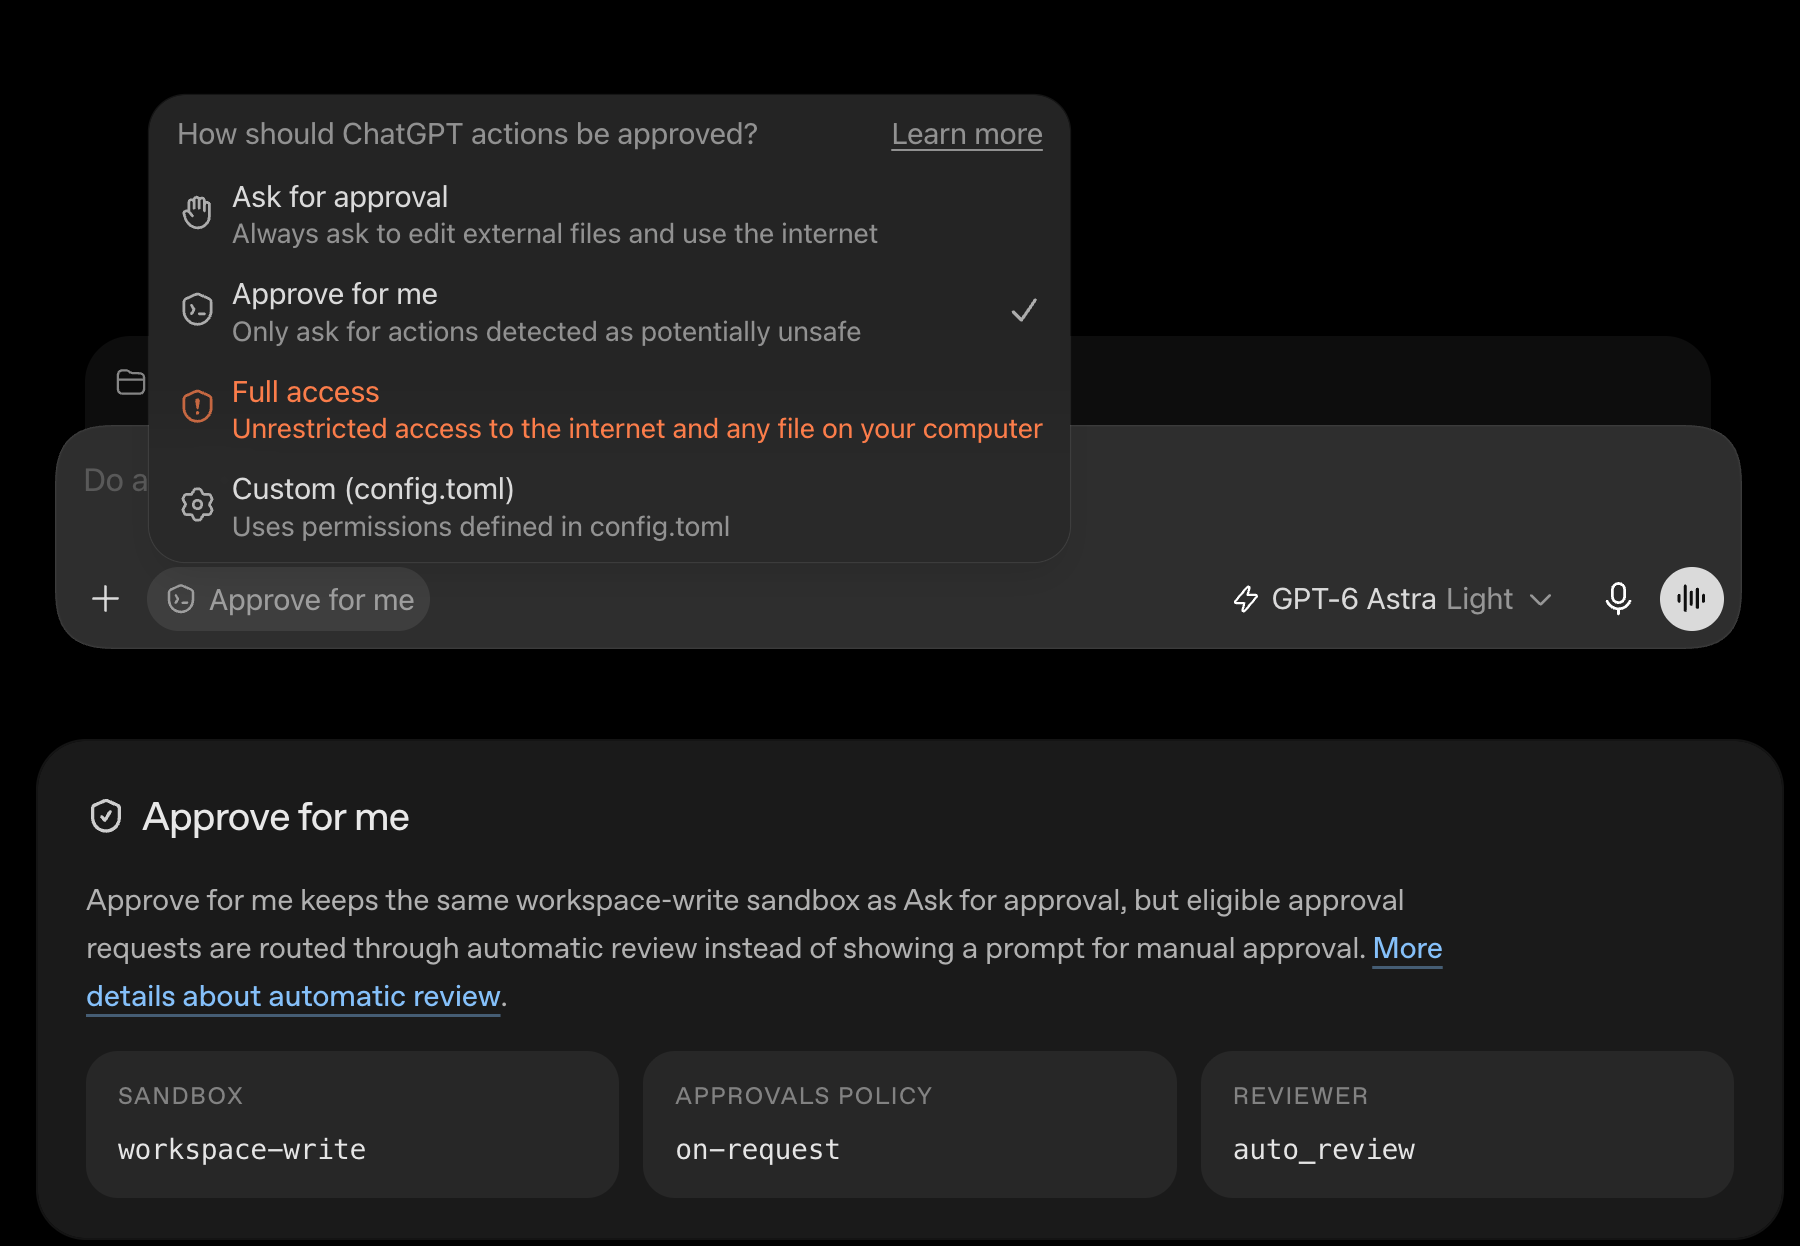
\includegraphics[width=173mm,trim=148bp 684bp 728bp 94bp,clip]{assets/selector-permisos.png}};
\texto{199}{124}{109}{14}{\textcolor{Azul}{\textbf{Ask for approval}}\\Revisión humana.}
\texto{199}{100}{109}{14}{\textcolor{Azul}{\textbf{Approve for me}}\\Revisión automática elegible.}
\texto{199}{76}{109}{14}{\textcolor{Violeta}{\textbf{Full access}}\\Sin fronteras del sandbox ni prompts.}
\texto{199}{48}{109}{14}{\textcolor{Azul}{\textbf{Custom}}\\Configuración personalizada.}
\texto{12}{20}{289}{10}{Captura del usuario. Opciones sujetas a cliente, cuenta y políticas.}

\note{La captura fue aportada por el usuario y muestra una selección histórica, no la configuración actual verificada. Ask for approval y Approve for me conservan workspace-write inicialmente y cambian el revisor elegible. La página define Full access como danger-full-access más never; no concede permisos de administrador del sistema. Custom o perfiles nombrados dependen del cliente y configuración. La captura se incluye como imagen real recortada en LaTeX. No es una instrucción para seleccionar Full access. Fuente oficial, consulta del 5 de noviembre de 2026: \refprincipal\ y \refauto.}

\end{scope}
\end{tikzpicture}
\end{frame}

\begin{frame}[plain]
\begin{tikzpicture}[remember picture,overlay,x=1mm,y=1mm]
\begin{scope}[shift={(current page.south west)}]
\pie{04 / Demo y apoyo}
\tit{Preferencias dentro de límites obligatorios}
\bajada{Tú eliges cómo empezar. La empresa limita qué opciones puedes elegir.}

\texto{22}{123}{128}{17}{\textcolor{Azul}{\textbf{Tu preferencia}}}
\texto{22}{109}{128}{12}{\texttt{config.toml}}
\texto{22}{94}{128}{12}{\texttt{sandbox\_mode = \textquotedbl workspace-write\textquotedbl}\\\texttt{approval\_policy = \textquotedbl on-request\textquotedbl}}
\texto{22}{69}{128}{12}{Escribir dentro del proyecto.\\Pedir aprobación para una excepción.}

\texto{173}{123}{129}{17}{\textcolor{Azul}{\textbf{Regla de la empresa}}}
\texto{173}{109}{129}{12}{\texttt{requirements.toml}}
\texto{173}{94}{129}{12}{\texttt{allowed\_sandbox\_modes = [}\\\texttt{\hspace{4mm}\textquotedbl read-only\textquotedbl,}\\\texttt{\hspace{4mm}\textquotedbl workspace-write\textquotedbl}\\\texttt{]}}
\texto{173}{64}{129}{12}{La empresa admite solo esos dos modos.}
\draw[Linea,line width=.5pt] (158,55) -- (158,127);

\regla{51}
\texto{22}{46}{142}{12}{\texttt{workspace-write} o \texttt{read-only}}
\texto{173}{46}{129}{12}{Compatibles con esta regla.}
\texto{22}{35}{142}{12}{\textcolor{Violeta}{\texttt{danger-full-access}}}
\texto{173}{35}{129}{12}{No se admite como opción permitida.}
\cierre{Tu preferencia debe estar dentro de las opciones que permite la empresa.}
\texto{12}{13}{295}{8}{Ejemplo con modos tradicionales. Para clientes recientes, OpenAI recomienda perfiles de permisos.}

\note{Ejemplo conceptual, no aplicado al sistema. config.toml selecciona workspace-write y on-request; requirements.toml limita los modos a read-only y workspace-write. Esa regla no impone por sí misma un valor a approval\_policy: el ejemplo solo muestra una restricción de modo. Elegir cualquiera de esos dos modos cumple esta regla específica, sin afirmar que satisfaga todas las demás políticas. danger-full-access queda fuera de la lista. La documentación vigente indica que, al resolver una configuración incompatible con un requisito, un cliente local compatible recurre a un valor compatible y avisa al usuario; no prometer un fallo universal de inicio. Este ejemplo conserva la familia tradicional usada por el resto del deck. OpenAI recomienda allowed\_permission\_profiles y default\_permissions para clientes recientes; no mezclar ambas familias en una configuración. MDM es un canal de gestión del dispositivo, no un tercer tipo de preferencia, y por eso se explica aquí: puede distribuir requisitos obligatorios. Las preferencias ordinarias tienen prioridades entre sí, pero deben respetar los requisitos efectivos, que también tienen su propia precedencia. Fuentes oficiales consultadas el 5 de noviembre de 2026: \url{https://learn.chatgpt.com/docs/enterprise/managed-configuration}\ y \refconfig. Diseño: ejemplo resuelto, interpretación junto al código y resultado explícito; adaptado de las orientaciones institucionales de \url{https://citral.ucsb.edu/faculty/resources/engaging-students/explaining-content}\ y \url{https://education.nsw.gov.au/about-us/education-data-and-research/cese/publications/practical-guides-for-educators/cognitive-load-theory-in-practice.html}.}

\end{scope}
\end{tikzpicture}
\end{frame}
\end{document}
